\subsection{Evaluation}

\subsubsection{Rank List Fusions Evaluation \label{sec:eval_fusion}}

In this experiment, the goal to understand if fusing rank lists can create better rank lists.
The methodology used, is to create $n$ isolated rank lists and fuse them for every $r$ rank lists combinations ($C^n_r$) for the two fusing methods proposed, Z-Score fusion and regression fusion.

The rank list used are the ones obtained by using the 9 retained rank list methods ($n=9$), see Table~\ref{tab:9rl}.
They represent the best configuration retained for each text representation.
The $r$ value is selected to $4$, since it represents the number of different text representation.
The number of possible fusion combinations with $n=9$ and $r=4$ is $C^{9}_{4} = 126$.
For these 126 fusions, the three following metrics are computed: Average Precision (AP), R-Precision (RPrec) and High Precision (HPrec).

To be able to compare the rank list produced by both the Z-Score fusions and the regression fusion to the non-fused rank lists (one to many), two evaluation strategies are used.
One called \textit{Single-Max} which represent the best metrics for each rank list in the fusion and another one called \textit{Single-Mean} which is represented by the mean of each rank list metrics in the fusion.

An example for these two comparison strategy is presented in Example~\ref{ex:single_mean_single_max}.

If the Single-Max evaluation strategy is over-come by a rank list produced by a fusion it means that the resulting rank list give results even better than every individual rank lists used for this fusion, this represents the best case where the fusion actually improve the results.
For the Single-Mean, if it is over come it means that the obtained rank list have better results than the average results of the rank list, thus when using the system \textit{in the blind} (when the rank list can't be evaluated, with new data for example), fusing is a good approach since it can give stability.

The results of every fusion combinations using the proposed rank list and strategies are graphically presented in Figure~\ref{fig:fusions}.
Statistics for each metric and fusion schemes are resumed Tables~\ref{tab:fusion_stats_A}/\ref{tab:fusion_stats_B}, it contains for each metric, the minimal value (min), the average and the standard deviation (Avg$\pm$Std), the maximal value, the argmin and argmax for the metrics (using ids of the rank list see Table~\ref{tab:9rl}).
A sign test between the two strategies and the two fusion methods is presented in Table~\ref{tab:fusion_sign_test}.

Using these distance metrics on St-jean, the sign test tends to indicate that the fusion increase the overall quality of the rank list.
The three evaluations metrics are high correlated (especially average precision and R-Precision), the average precision is used as a foundation for the analysis.
The Z-Score fusion, produce for every metrics better results than both Single-Mean and Single-Max, the average precision is increase in average by $\sim 10$\% compared to the average of the average precision (Single-Mean) of the rank list used, and by ~6\% in average when considering the maximal average precision (Single-Max).
In the other hand, the Regression fusion, have an average increase of $\sim 3$\% in average precision for the Single-Mean and have a decrease of ~1\% when comparing to the Single-Max.
The standard deviation of the regression fusion is greater than the Z-Score fusion, this indicates a slightly greater instability in the results.
A general observation of the Tables~\ref{tab:fusion_stats_A} and \ref{tab:fusion_stats_B} and Figure~\ref{fig:fusions}, show that the HPrec tends to be the least easy metric to increase when using the fusion.
The results of fusing multiple rank lists when using regression fusion strategy tends to indicate that the resulting rank list has in average an equivant quality as the best rank list used for the fusion with some slight decreases.
This can be further confirmed by looking at Table~\ref{tab:fusion_B}, which shows in the column Regression/T/Single-Max more ties and in Figure~\ref{fig:fusions} where most Regression score and Single rank list score some overlap.
No particular set of rank list tends to give the best results in every case when fusing with the two strategies, every rank list is present in the argmax, but with the Z-Score fusion, the best results are obtained with rank lists using different text representations.
The Z-Score fusion give the best results overall.

\begin{figure}
  \centering
  \caption{Evaluation of every combination of 4 rank list fusions using Z-Score and Regression}
  \label{fig:fusions}

  \subcaption{Testing on St-Jean A (training St-Jean B, for the Regression fusion)}
  \label{fig:fusion_evaluation_A}
  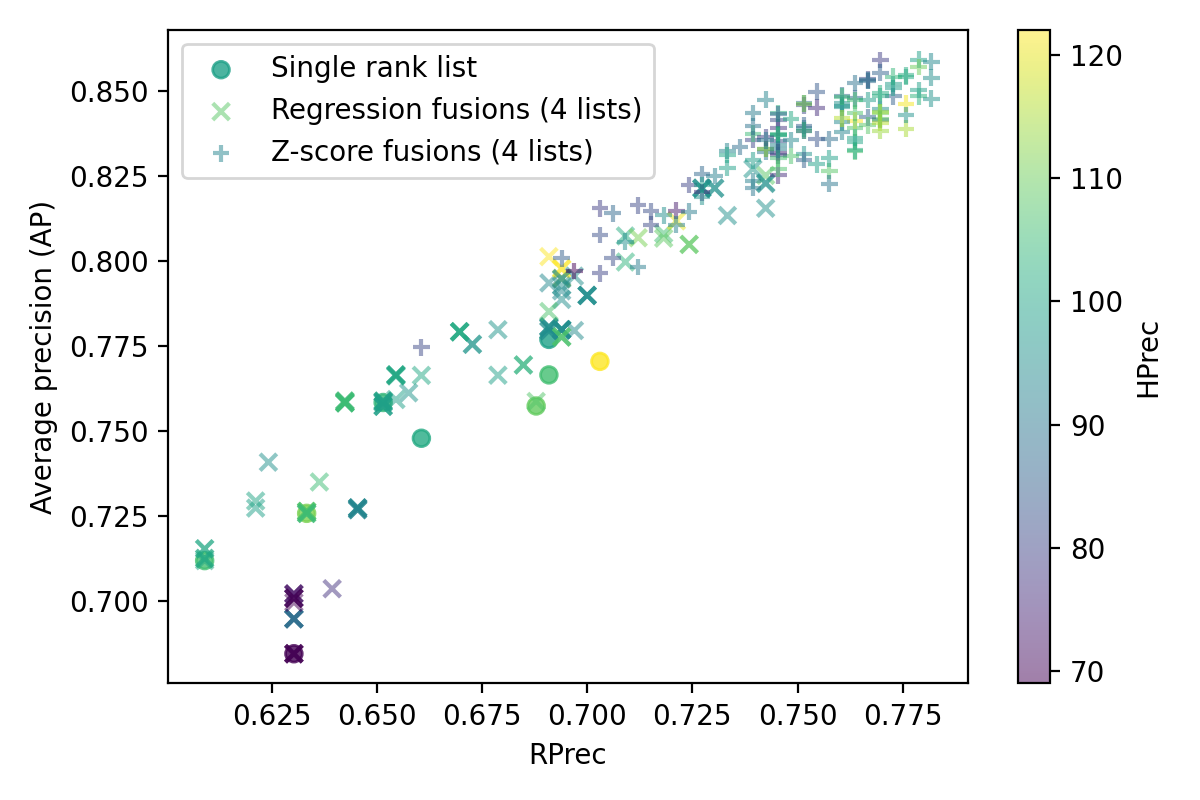
\includegraphics[width=\linewidth]{img/fusion_evaluation_A.png}

  \vspace{0.5cm}

  \subcaption{Testing on St-Jean B (training St-Jean A, for the Regression fusion)}
  \label{fig:fusion_evaluation_B}
  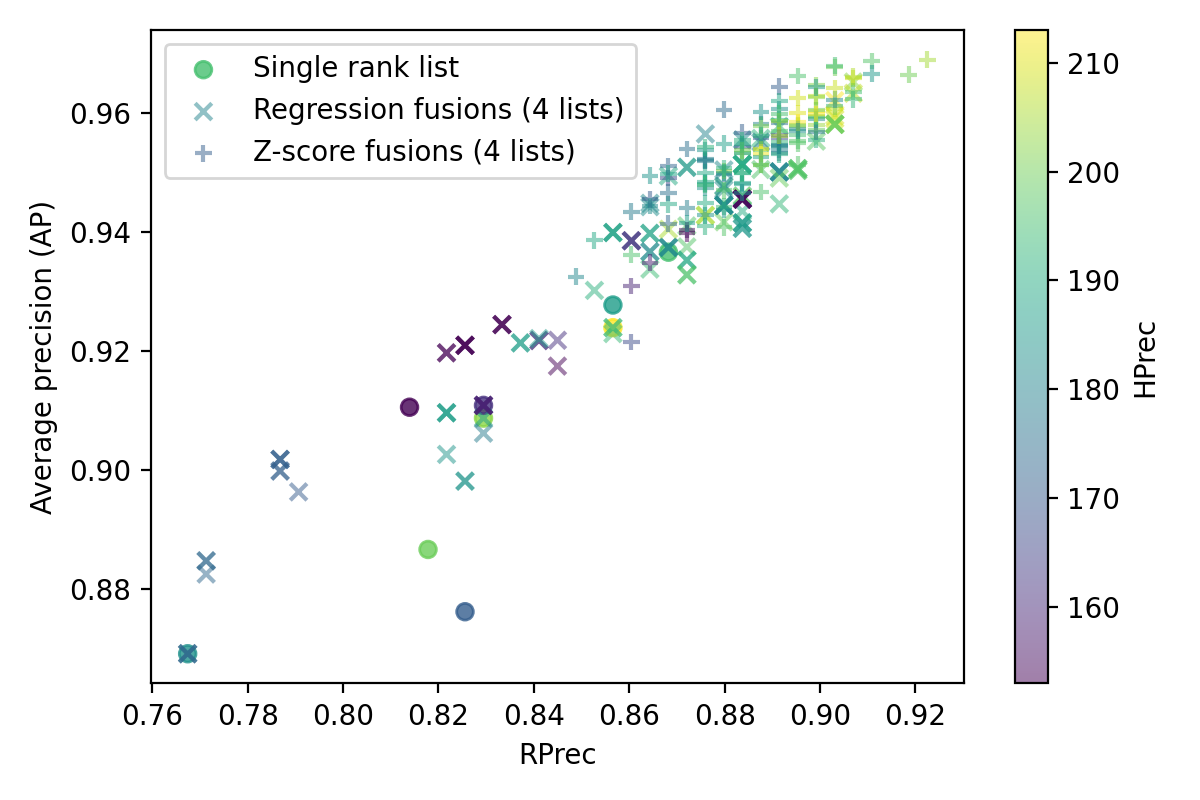
\includegraphics[width=\linewidth]{img/fusion_evaluation_B.png}
\end{figure}

\begin{table}
  \centering
  \caption{Fusion statistics on St-Jean A}
  \label{tab:fusion_stats_A}

  \subcaption{Single-Mean}
  \resizebox{\linewidth}{!}{
  \begin{tabular}{l l l l}
    \toprule
    Stats
    & AP
    & RPrec
    & HPrec \\
    \midrule
    Min & $0.72$ & $0.63$ & $56.25$ \\
    Avg$\pm$Std & $0.74\pm0.01$ & $0.66\pm0.01$ & $70.78\pm8.00$ \\
    Max & $0.77$ & $0.69$ & $84.25$ \\
    Argmin & [1,4,6,7] & [4,5,6,7] & [0,1,5,7] \\
    Argmax & [0,2,5,8] & [0,2,3,8] & [2,3,4,6] \\
    \bottomrule
  \end{tabular}
  }

  \vspace{0.5cm}

  \subcaption{Single-Max}
  \resizebox{\linewidth}{!}{
  \begin{tabular}{l l l l}
    \toprule
    Stats
    & AP
    & RPrec
    & HPrec \\
    \midrule
    Min & $0.75$ & $0.65$ & $72.00$ \\
    Avg$\pm$Std & $0.77\pm0.01$ & $0.69\pm0.01$ & $88.66\pm9.55$ \\
    Max & $0.78$ & $0.70$ & $99.00$ \\
    Argmin & [1,4,6,7] & [4,5,6,7] & [0,1,5,7] \\
    Argmax & [0,1,2,3] & [0,1,2,3] & [0,1,2,3] \\
    \bottomrule
  \end{tabular}
  }

  \vspace{0.5cm}

  \subcaption{Z-Score}
  \resizebox{\linewidth}{!}{
  \begin{tabular}{l l l l}
    \toprule
    Stats
    & AP
    & RPrec
    & HPrec \\
    \midrule
    Min & $0.77$ & $0.66$ & $69.00$ \\
    Avg$\pm$Std & $0.84\pm0.02$ & $0.75\pm0.02$ & $93.92\pm11.15$ \\
    Max & $0.86$ & $0.78$ & $122.00$ \\
    Argmin & [0,4,5,7] & [0,4,5,7] & [0,1,4,5] \\
    Argmax & [0,3,6,7] & [0,3,4,8] & [0,3,7,8] \\
    \bottomrule
  \end{tabular}
  }

  \vspace{0.5cm}

  \subcaption{Regression (training St-Jean B)}
  \resizebox{\linewidth}{!}{
  \begin{tabular}{l l l l}
    \toprule
    Stats
    & AP
    & RPrec
    & HPrec \\
    \midrule
    Min & $0.68$ & $0.61$ & $20.00$ \\
    Avg$\pm$Std & $0.76\pm0.04$ & $0.67\pm0.04$ & $68.84\pm19.41$ \\
    Max & $0.83$ & $0.74$ & $112.00$ \\
    Argmin & [2,3,7,8] & [1,2,4,8] & [2,3,4,7] \\
    Argmax & [0,1,2,6] & [0,1,2,3] & [0,1,3,7] \\
    \bottomrule
  \end{tabular}
  }
\end{table}

\begin{table}
  \centering
  \caption{Fusion statistics on St-Jean B}
  \label{tab:fusion_stats_B}

  \subcaption{Single-Mean}
  \resizebox{\linewidth}{!}{
  \begin{tabular}{l l l l}
    \toprule
    Stats
    & AP
    & RPrec
    & HPrec \\
    \midrule
    Min & $0.89$ & $0.81$ & $137.50$ \\
    Avg$\pm$Std & $0.91\pm0.01$ & $0.83\pm0.01$ & $154.89\pm7.22$ \\
    Max & $0.92$ & $0.85$ & $172.00$ \\
    Argmin & [3,4,6,8] & [1,3,6,8] & [1,6,7,8] \\
    Argmax & [0,2,5,7] & [0,2,5,7] & [0,3,4,5] \\
    \bottomrule
  \end{tabular}
  }

  \vspace{0.5cm}

  \subcaption{Single-Max}
  \resizebox{\linewidth}{!}{
  \begin{tabular}{l l l l}
    \toprule
    Stats
    & AP
    & RPrec
    & HPrec \\
    \midrule
    Min & $0.91$ & $0.83$ & $153.00$ \\
    Avg$\pm$Std & $0.93\pm0.01$ & $0.86\pm0.01$ & $174.75\pm7.29$ \\
    Max & $0.94$ & $0.87$ & $182.00$ \\
    Argmin & [3,4,6,8] & [1,3,6,8] & [1,6,7,8] \\
    Argmax & [0,1,2,3] & [0,1,2,3] & [0,1,2,5] \\
    \bottomrule
  \end{tabular}
  }

  \vspace{0.5cm}

  \subcaption{Z-Score}
  \resizebox{\linewidth}{!}{
  \begin{tabular}{l l l l}
    \toprule
    Stats
    & AP
    & RPrec
    & HPrec \\
    \midrule
    Min & $0.92$ & $0.85$ & $153.00$ \\
    Avg$\pm$Std & $0.95\pm0.01$ & $0.89\pm0.01$ & $188.91\pm12.87$ \\
    Max & $0.97$ & $0.92$ & $213.00$ \\
    Argmin & [2,3,6,8] & [3,4,6,8] & [1,2,3,6] \\
    Argmax & [1,2,5,7] & [1,2,5,7] & [0,3,4,7] \\
    \bottomrule
  \end{tabular}
  }

  \vspace{0.5cm}

  \subcaption{Regression (training St-Jean A)}
  \resizebox{\linewidth}{!}{
  \begin{tabular}{l l l l}
    \toprule
    Stats
    & AP
    & RPrec
    & HPrec \\
    \midrule
    Min & $0.87$ & $0.77$ & $124.00$ \\
    Avg$\pm$Std & $0.93\pm0.02$ & $0.86\pm0.04$ & $165.25\pm22.09$ \\
    Max & $0.97$ & $0.91$ & $210.00$ \\
    Argmin & [2,3,6,8] & [2,3,6,8] & [1,2,3,8] \\
    Argmax & [0,1,2,7] & [0,1,2,7] & [0,1,3,7] \\
    \bottomrule
  \end{tabular}
  }
\end{table}

\begin{table*}
  \centering
  \caption{Rank list fusion sign test. \textit{The star (*) indicate a Binomial test p-value smaller than 5\%}, S-Mean: Single-Mean, S-Max: Single-Max}
  \label{tab:fusion_sign_test}

  \subcaption{Testing St-Jean A (training St-Jean B, for the Regression fusion)}
  \label{tab:fusion_A}
  \begin{tabular}{l c c c c}
    \toprule
    Metric
    & Z-Score/Tie/S-Mean
    & Z-Score/Tie/S-Max
    & Regression/Tie/S-Mean
    & Regression/Tie/S-Max \\
    \midrule
    AP    & *126/0/0 & *125/0/1 & *85/0/41 & 58/0/68 \\
    RPrec & *126/0/0 & *124/1/1 & 66/1/59  & 38/7/81* \\
    HPrec & *124/0/2 & *77/4/45 & 58/1/67  & 16/5/105*\\
    \bottomrule
  \end{tabular}

  \vspace{0.5cm}

  \subcaption{Testing St-Jean B (training St-Jean A, for the Regression fusion)}
  \label{tab:fusion_B}
  \begin{tabular}{l c c c c}
    \toprule
    Metric
    & Z-Score/Tie/S-Mean
    & Z-Score/Tie/S-Max
    & Regression/Tie/S-Mean
    & Regression/Tie/S-Max \\
    \midrule
    AP    & *126/0/0 & *125/0/1  & *116/0/10 & *87/0/39 \\
    RPrec & *126/0/0 & *123/2/1  & *103/1/22 & *72/11/43 \\
    HPrec & *126/0/0 & *108/2/16 & *87/1/38  & 43/9/74*\\
    \bottomrule
  \end{tabular}

\end{table*}

\subsubsection{Veto Evaluation}

In this experiment, the goal is to understand if the veto method can improve the average precision on the fused rank lists when using the regression fusion method.
To do so, the St-Jean retained rank list are used (ref. Table~\ref{tab:9rl_results_st_jean} in annex).
The fusion scheme is learnt on first St-Jean A and trained on St-Jean B (ref. Section~\ref{sec:regression_fusion}), then the inverse.
After computing the probabilities for each link in each rank list on the testing set, the probabilities under the threshold are set according to each proposed veto strategy (set to $0$, $-1$, $-n$, $-\infty$).
The threshold is analysed for the values between $0.01$ and $0.50$, with a step of $0.01$.
A threshold of $0.50$ is an upper bound, after this value the probability of being a false link is smaller than the probability of being a true link, thus having a veto on a link more likely to be true link than false link is a bad idea.
The fusion of the rank list is normally computed with the average of the probabilities with one small difference for the $-\infty$ strategy when a $-\infty$ is encountered in the mean, the mean will always be $-\infty$.
To understand if the veto improve the results, the average precision gain of the rank list between the veto strategy and without the veto.

The average precision difference over the threshold value is visually presented in Figure~\ref{fig:veto}, and the best configurations found are summarized in Table~\ref{tab:veto}.
Overall, the veto strategy seem to be a bad option.
The best result obtained is only a gain of 0.0193 average precision, with a tiny threshold (0.01, the closest to a non threshold approach) which may indicate an increase due to random factors.
Using the $-\infty$ strategy only give worse results.
A possible reason why the veto fail to improve the results is that the veto strategy is only impactful when most of the rank lists rank a false link at the top except one rank list which correctly identify this false link and rank him at the bottom.
The rank list used for the experiment do not have such special cases since most of them correct classify false link at the bottom and true links at the top.
This strategy may be appliable on harder corpus such as the PAN 16 corpus.

\begin{figure}
  \caption{Veto strategies evaluations on St-Jean A and B depending on the threshold}
  \label{fig:veto}
  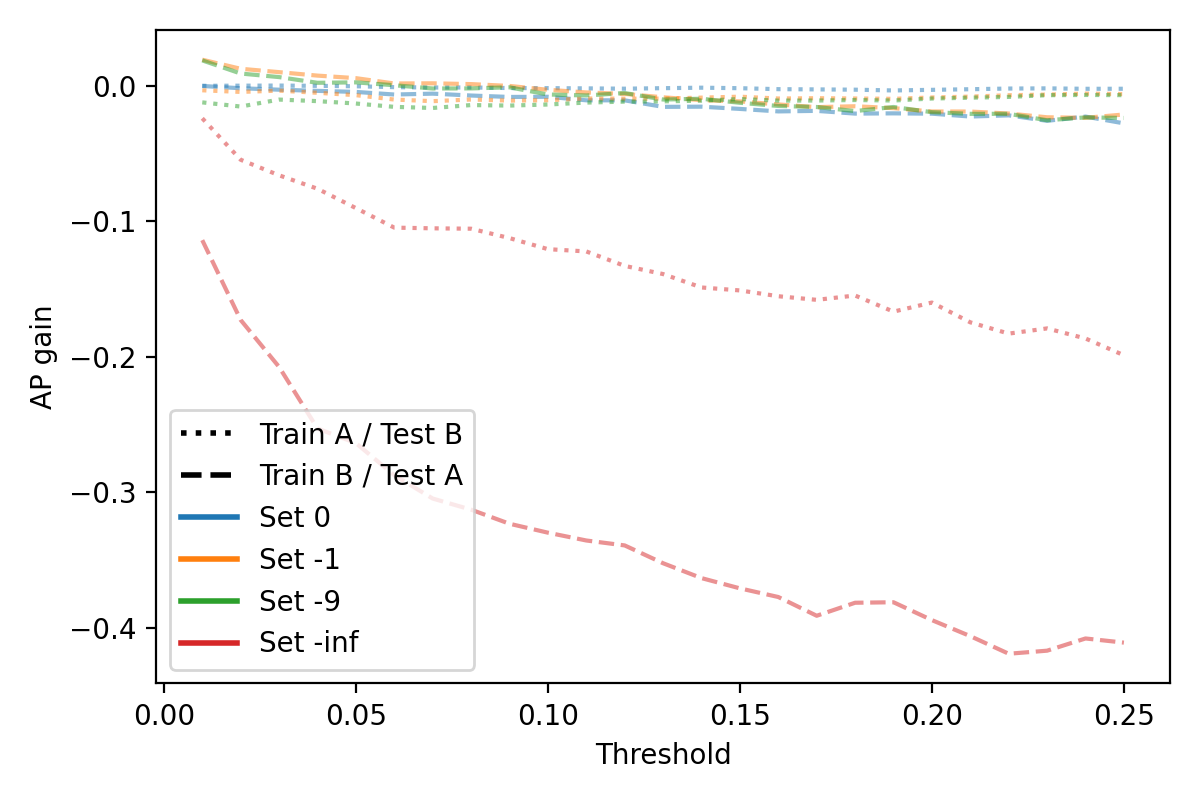
\includegraphics[width=\linewidth]{img/veto.png}
\end{figure}

\begin{table}
  \centering
  \caption{Maximal gain on the average precision using the veto / Argmax}
  \label{tab:veto}
  \begin{tabular}{l r r}
    \toprule
                   & Train A / Test B & Train B / Test A \\
    \midrule
    Set to $0$     & 1.98e-04/0.03 & -9.11e-05/0.01 \\
    Set to $-1$    & -3.28e-03/0.01 & 1.93e-02/0.01 \\
    Set to $-n$    & -6.73e-03/0.24 & 1.88e-02/0.01 \\
    Set to $-\inf$ & -2.40e-02/0.01 & -1.14e-01/0.01 \\
    \bottomrule
  \end{tabular}
\end{table}

\subsubsection{Soft-veto Evaluation}

To evaluate the performance of the soft veto strategy, the idea is to compute the average precision gain obtained when using the soft-veto over the simple fusion without it.
The gain is computed by subtracting the average precision of the Z-Score fusion without the soft-veto to the average precision of the Z-Score fusion with the soft-veto.
The soft-veto has two parameters : $c$ and $r$, to be able to find the best parameters the grid search approach is used.
Since the $c$ parameter must be in the interval $\left]0, \infty\right[$ and the $r$ parameter must be in the interval $\left]0, \infty\right[$, the grid is constructed from the Cartesian product of the following two sets.
$c = \left\{0 + \epsilon, 1, 2, 3, ..., 19, 20\right\}$, with $\epsilon$ a small value (for example $10^{-6}$) and $r = \left\{0.10, 0.14, 0.18, 0.22, ..., 0.86, 0.90\right\}$.
When computing the soft-veto gain using the grid search on the retained rank lists from Oxquarry (see Table~\ref{tab:9rl}), Figure~\ref{fig:soft_veto} is obtained.

The best parameters are c=18 and r=0.14 with an average precision gain of 3.50e-04.
As for the veto experiment, no real average precision gain can be obtained using this strategy since the average precision gain is small and can be due to random factors.

\begin{figure}
  \caption{Average precision gain with soft veto s-curve on Oxquarry}
  \label{fig:soft_veto}
  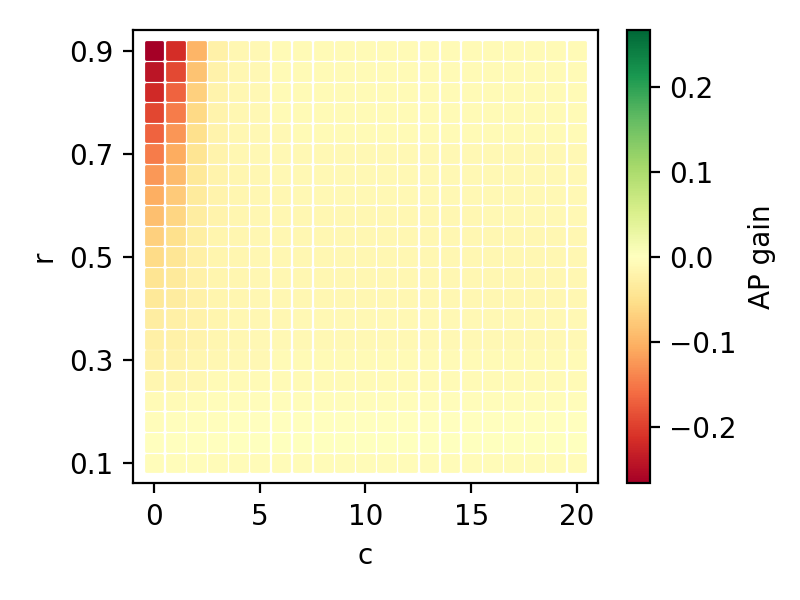
\includegraphics[width=\linewidth]{img/soft_veto.png}
\end{figure}

\subsubsection{Average precision fusion gain relation with the rank lists diversity}

As stated previously, we believe fusing high quality rank lists (high AP), with the most diverse results can increase the quality of the fusion.
First, a correlation metric to compare the rank lists must be selected.
And second compare the correlation coefficient to the average precision gain to verify the assumption.

To compute a correlation between two rank lists, the Kendall rank correlation coefficient is used~\cite{scipy}.
The Kendall rank correlation computes a correlation index based on the ordinal association between the two rank lists ranks by computing the difference in terms of number of swaps needed to sorts the rank lists ranks of the two lists.

The default weighing strategy called \textit{hyperbolic weighing} is used, it favours top ranks in the same fashion as the reciprocal rank ($1 / (r + 1)$).
The Kendall coefficient is ranged between -1 and 1, with 1 being an identical correlation and -1 a completely different correlation.
If our assumption is correct, the average precision gain obtained by fusing two rank lists should be negatively correlated to the rank list Kendall correlation coefficient.
A large gain, when the rank lists are different, thus a low rank list correlation coefficient, and vice versa.

The fusion strategy used here is the Z-Score fusion, since this strategy is parameterless and obtained satisfying results during previous experiments.
As for previous experiments dealing with fusion, the gain in average precision when comparing a set of rank list to a fused rank list can be established in the two following ways : \textit{Single-Mean} and \textit{Single-Max}.
Single-Mean represent the rank lists mean average precision and Single-Max the rank list maximal average precision.
Example~\ref{ex:single_mean_single_max} contain a small example with two rank lists for the Single-Mean and Single-Max methods to compute the average precision gain.

Table~\ref{tab:rl_correlations} show the Kendall correlation coefficient for every combination of retained rank list in St-Jean (see Table~\ref{tab:9rl}).
The most similar rank list pair are the two rank list using letters $n$-grams (0.95), least similar are the BZip2 compression and the 250-MFW POS (0.66).
For every pair of retained rank lists in St-Jean the Single-Mean fusion gain is computed and is compared to the distance in Figure~\ref{fig:rl_correlations}.
Using the linear regression, the best line for these point is computed~\cite{scipy}.
Reproducing this experiment for every corpus and fusion gain computation methods, the results are in Table~\ref{tab:rl_correlations_regression}.

For all experiment the linear correlation coefficient, $r$-value, is negative, which indicate that the average precision gain is negatively correlated to the Kendall correlation coefficient between the rank lists.
Thus, the assumption that suggested that the more diverse the rank lists are, the higher the quality of the fusion, seem to be confirmed.
The $p$-value for the linear regression (null hypothesis: the slope is 0) obtained after the regression is below 5\% for every of the Single-Mean experiments and for the Single-Max St-Jean corpus.
A clear linear relationship between the average precision gain and rank list diversity is observed on these datasets / average precision gain computation method.
Using the Single-Max strategy on Oxquarry and Brunet give a p-value of 15.1\% and 7.04\% respectively which can indicate that the linear correlation between the average precision gain and the diversity of the rank list can be obtained by random factors on these datasets with this comparison strategy.

Since the Single-Mean average precision gain follow a linear model, the gain can be predicted from the Kendall correlation coefficient. It's also possible to optimise the gain directly from the Kendall correlation coefficient, the lowest the correlation coefficient the greater the Single-Mean gain will be.
Knowing the average precision of rank lists it is possible to estimate Single-Mean gain with a linear model.
On main draw back is that the rank list used have to be known has good rank list already, since bad rank list will have a large Kendall correlation coefficient when compared to good rank lists but won't give good results when fused.

\begin{table}
  \centering
  \caption{Pairwise Kendall correlation coefficient on the retained rank lists St-Jean}
  \label{tab:rl_correlations}
  \resizebox{\linewidth}{!}{
  \begin{tabular}{r|r r r r r r r r}
    \toprule
    id &    1 &    2 &    3 &    4 &    5 &    6 &    7 &    8 \\
    \midrule
    0  & 0.86 & 0.83 & 0.80 & 0.88 & 0.91 & 0.73 & 0.81 & 0.75 \\
    1  &    - & 0.87 & 0.83 & 0.80 & 0.83 & 0.79 & 0.73 & 0.77 \\
    2  &    - &    - & 0.84 & 0.78 & 0.80 & 0.82 & 0.72 & 0.79 \\
    3  &    - &    - &    - & 0.78 & 0.81 & 0.80 & 0.75 & 0.85 \\
    4  &    - &    - &    - &    - & 0.95 & 0.77 & 0.81 & 0.75 \\
    5  &    - &    - &    - &    - &    - & 0.78 & 0.82 & 0.77 \\
    6  &    - &    - &    - &    - &    - &    - & 0.66 & 0.79 \\
    7  &    - &    - &    - &    - &    - &    - &    - & 0.82 \\
    \bottomrule
  \end{tabular}
  }
\end{table}

\begin{figure}
  \centering
  \caption{Fusion average precision gain (using Single-Mean scheme) over rank list distance on St-Jean}
  \label{fig:rl_correlations}
  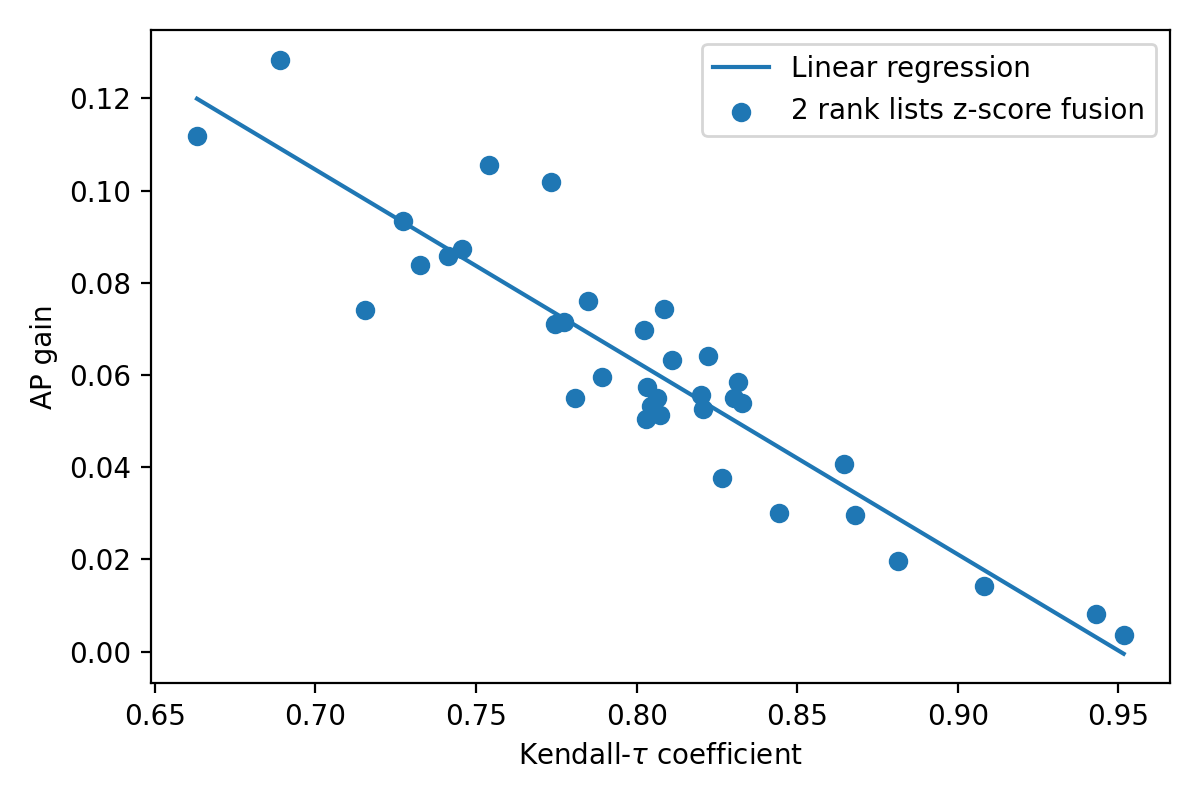
\includegraphics[width=\linewidth]{img/rank_list_correlation_mean_st_jean.png}
\end{figure}

\begin{table}
  \centering
  \caption{Linear regression on the average precision gain over Kendall r-coefficient}
  \label{tab:rl_correlations_regression}

  \subcaption{Single-Mean}
  \begin{tabular}{l r r r r r}
    \toprule
    Corpus/Method & $r$-value & $p$-value & Std. error \\
    \midrule
    Oxquarry & -0.63 & 2.04e-03 & 4.36e-02 \\
    Brunet   & -0.89 & 7.14e-08 & 2.17e-02 \\
    St-Jean  & -0.93 & 9.30e-17 & 2.49e-02 \\
    \bottomrule
  \end{tabular}

  \vspace{0.5cm}

  \subcaption{Single-Max}
  \begin{tabular}{l r r r r r}
    \toprule
    Corpus/Method & $r$-value & $p$-value & Std. error \\
    \midrule
    Oxquarry  & -0.32 & 1.51e-01 & 8.15e-02 \\
    Brunet    & -0.40 & 7.04e-02 & 4.50e-02 \\
    St-Jean   & -0.86 & 1.60e-11 & 3.72e-02 \\
    \bottomrule
  \end{tabular}
\end{table}
